\documentclass[12pt, letterpaper]{article}
\usepackage[hyphens]{url}
\setlength{\topmargin}{-1.75cm} \setlength{\textheight}{22.5cm}
\setlength{\oddsidemargin}{0.25cm}
\setlength{\evensidemargin}{0.25cm} \setlength{\textwidth}{16.2cm}
\renewcommand{\figurename}{Figure}
\usepackage{amssymb}
\usepackage{graphicx}
\usepackage{amsmath}
\usepackage{xcolor}
\usepackage[normalem]{ulem}
\usepackage{fontenc}
\usepackage{footnote}
\usepackage[breaklinks]{hyperref}
\usepackage{palatino, multicol, listings} % for multiple columns
\lstset{mathescape=true, basicstyle=\ttfamily,}

%\usepackage{pictex}
%% in the .pictex output of xfig, there is command \colo
%% however the old version of pictex may not define this
%% so we define color here as empty
%\def \color#1]#2{}

\begin{document}

\newcommand{\hide}[1]{}
\newcommand{\exercise}[1]{}
\newcommand{\future}[1]{}
\newcommand{\otherquestions}[1]{}
\newcommand{\set}[1]{\{#1\}}
\newcommand{\pg}[1]{{\tt #1}}
\newtheorem{definition}{Definition}
\newcommand{\emptyclause}{\Box}
\def\st{\bigskip\noindent}
\newcommand{\lplus}
{
   \stackrel{+}{\gets}
}

\newcommand{\fe}[1] {
  \begin{frame}
    #1
  \end{frame}}

\newcommand{\eoa}{ {\bf End} of algorithm}

\newcommand{\ft}[1] {\frametitle{#1}}

\newcommand{\ie}[1] {
  \begin{itemize}
    #1
  \end{itemize}
}

\newcommand{\ee}[1] {
  \begin{enumerate}
    #1
  \end{enumerate}\label{marker}
}
\newcommand{\blk}[2] {
  \begin{block}{#1}
    #2
  \end{block}
}

\newtheorem{collorary}{Corollary}
\newtheorem{proposition}{Proposition}
\newtheorem{invariant}{Invariant}
\newtheorem{property}{Property}
\newtheorem{claim}{Claim}
\newtheorem{example}{Example}


\title{${\cal SPARC}$ manual}
\date{\today}
\maketitle
\tableofcontents
\pagebreak


\section{System installation}

\st For using the system, you need to have the following installed:
\begin{enumerate}
\item Java Runtime Environment (JRE) can be found at \\
{\scriptsize
\url{http://www.oracle.com/technetwork/java/javase/downloads/jre8-downloads-2133155.html}
}.\\
Java versions 1.8.0\_181 or higher is required.
\item The SPARC to ASP translator. It can be downloaded at \\ 
{\scriptsize
\url{https://github.com/iensen/sparc/blob/master/sparc.jar?raw=true}
}.
\item An ASP solver. It can be one of the following:
  \begin{enumerate}
  \item Clingo (recommended)  {\scriptsize
 \url{https://github.com/potassco/clingo/releases}
}.
\item DLV
{\scriptsize
 \url{http://www.dlvsystem.com/dlv/#1}
}. You need to download the \textit{static} version of the executable file.

\end{enumerate}

\item (\textit{optional}) Swi-Prolog. {\scriptsize \url{http://www.swi-prolog.org/}}. This item is only required if option \textit{-wcon} is used for type warning detection.
(See sections \ref{option} and \ref{clp_type_warnings}).

\end{enumerate}
If you are using the dlv solver, rename the solver executable file to \textit{dlv} (\textit{dlv.exe} for windows).

Be sure the PATH system variable includes the directory where the solver executable is located. For instructions on how to view/modify the PATH system variable, see either of the following links:\\
{\scriptsize
\url{http://www.java.com/en/download/help/path.xml}\\
\url{http://www.cyberciti.biz/faq/appleosx-bash-unix-change-set-path-environment-variable/}\\
}
To check if the solver is installed correctly, run the command \texttt{dlv -v} (for dlv) or \\ \texttt{clingo -v} (for clingo). See figures \ref{fig:dlv_solver_check} for dlv and \ref{fig:clingo_solver_check} for clingo for examples of the expected output.

\begin{figure}[p]
\centering
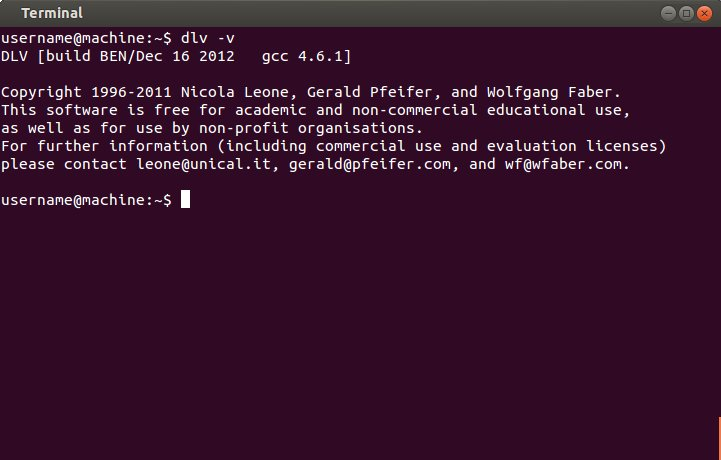
\includegraphics[width=0.9\textwidth]{dlv_version.jpg}
\caption{Checking the version of DLV solver}
\label{fig:dlv_solver_check}
\end{figure}


\begin{figure}[p]
\centering
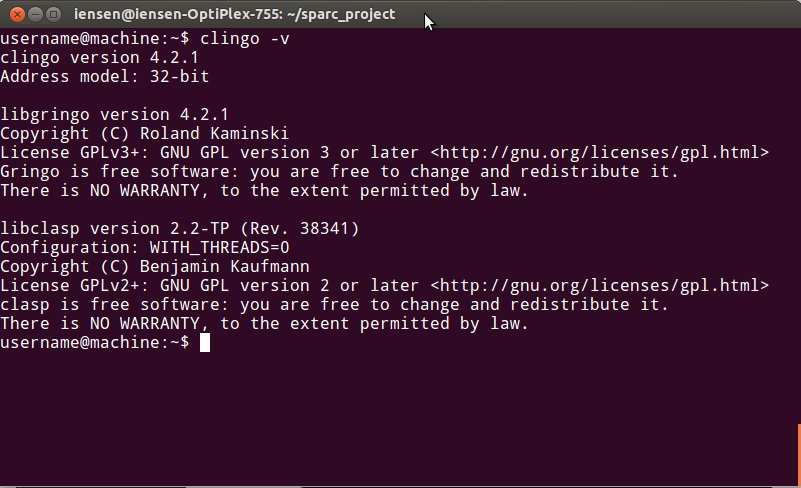
\includegraphics[width=0.9\textwidth]{clingo_version.jpg}
\caption{Checking the version of Clingo solver}
\label{fig:clingo_solver_check}
\end{figure}

\section{System usage}

To demonstrate the usage of the system we will use the program $\Pi$ below.
\begin{verbatim}
sorts
#person={bob,tim,andy}.
predicates
teacher(#person).
rules
teacher(bob).
\end{verbatim}

\st
The system can work in one of the  two modes: \textit{querying mode} and \textit{answer set mode}.

\subsection{Querying mode}

In this mode we can ask queries about a ${\cal SPARC}$ program loaded into the system.
The general command line syntax for this mode is \textit{java -jar sparc.jar program\_file}.
Queries in ${\cal SPARC}$ are positive or negative literals of the forms $p(t1,t2,\dots,tn)$ or
$-p(t1,t2,\dots,tn)$ correspondingly, where $p(t1,t2,\dots,tn)$  is an atom of the loaded program $\Pi$ 
( note that \textit{n} can be equal to zero, in this case the query will be of the form \textit{p} or \textit{-p}  ).

The queries are answered as follows:
\ie{
\item The answer to a query $l$ not containing variables is \textit{yes}, if $l$(with all arithmetic expressions evaluated) belongs to all answer sets of  $\Pi$.
\item The answer to a query $l$ not containing variables is \textit{no}, if $-l$(with double classical negation removed and all arithmetic expressions evaluated) belongs to all answer sets of  $\Pi$.
\item The answer to a query $l$ not containing variables is \textit{unknown}, if it is not \textit{yes} or \textit{no}.
\item The answer to a query of the form $l$($l$ is an atom of the form $p(t1, \dots, tn)$  possibly preceeded by a negation sign)  is  a collection of assignments $X_1 = t_1, \dots, X_n=t_n$,
where $X_1, \dots, X_n$ are all variables in $p(t1, \dots, tn)$, $t_1, \dots, t_n$ are ground terms, and the answer to the query $p(t1',\dots,tn')$, obtained from  $p(t1, \dots, tn)$ by replacing each variable $X_i$ by a ground term $t_i$, is \textit{yes}.

}

To run  ${\cal SPARC}$  on the program above, 
we change current directory to a directory having the file \texttt{program.sp} with the program written in it, and the downloaded file \texttt{sparc.jar}.  Then, we run the command:
\begin{verbatim}
username@machine:~$ java -jar sparc.jar program.sp
SPARC  V2.25
program translated
?- teacher(bob).
yes
?- teacher(tim).
unknown
?- teacher(X).
X = bob
?- teacher(john).
program.sp: argument number 1 of predicate teacher/1, "john", 
            violates definition of sort "person"
?-exit.
\end{verbatim}

The answer to the first query \texttt{?- teacher(bob)} is \textit{yes}, because the atom \textit{teacher(bob)} belongs to the only answer set of $\Pi$.

The answer to the second query \texttt{?- teacher(tim)} is \textit{unknown}, because neither the atom \textit{teacher(bob)} nor its negation belongs to the answer set of $\Pi$.

The answer to the query \texttt{?- teacher(X)} is \textit{X = bob}, because there is only one replacement (bob) for X, such that \textit{teacher(X)} belongs to the answer set of $\Pi$.

For the fourth query, we see an error, because teacher(john) is not an atom of $\Pi$.

To quit the querying engine, use \textbf{exit} command.

\subsection{Answer Set Mode}

In this mode we can see the computed answer sets of the loaded program.
The general command line syntax for this mode is \textit{java -jar sparc.jar program\_file -A}.

For the program $\Pi$, the answer set may be computed as it is shown below:
\begin{verbatim}
username@machine:~$ java -jar sparc.jar program.sp -A
SPARC  V2.25
program translated
DLV [build BEN/Dec 16 2012   gcc 4.6.1]
{teacher(bob)}

\end{verbatim}

\section{Command Line Options}\label{option}

In this section we  describe the meanings of command line options supported by
${\cal SPARC}$. Some options(flags) do not take an argument and have the form \textit{-option},
while others require arguments and can be written in the form \textit{-option arg}.
For each command line option, we indicate whether it requires
an argument, and if so, we  describe its meaning.

\begin{itemize}
 \item \textbf{-A}
    
  Compute answer sets of the loaded program.

\item \textbf{-wcon}
    
  Show warnings determined by CLP-based algorithm. See section \ref{clp_type_warnings}

\item \textbf{-wasp} 
  \footnote{\textcolor{red}{This option is temporarily broken, use -wcon instead}}
  Show warnings determined by ASP-based algorithm. See section \ref{asp_type_warnings}

\item \textbf{-solver arg}
  Specify the solver which will be used for computing answer sets. \textit{arg} can have two possible values: \textit{dlv} and \textit{clingo}. 
\item \textcolor{red}{(\textbf{new!})} \textbf{-n [number]}

  Specify how many answer sets need to be displayed. This option can only be used with option -A.
  
  Examples:
  \begin{itemize}
  \item[$\bullet$] \texttt{-n 2} will display two arbitrary answer sets. In case the program has less than two answer sets, all of them will be shown.
  \item[$\bullet$] \texttt{-n 0} will display all the answer sets.
    \end{itemize}


\item \textbf{-Help, -H, -help, --Help, --help, -h}

  Show help message.

\item \textbf{-o arg}

  Specify the output file where the translated ASP program will be written. \textit{arg} is the path to the output file. 
  Note that if the option is not specified, the translated ASP program will not be stored anywhere.

\item \textbf{input\_file}
  
Specify the file where the sparc program is located.



\end{itemize}


\section{Syntax Description}

\subsection{Directives}
Directives should be written before sort definitions, at the very beginning of a program.
${\cal SPARC}$ allows two types of directives:
\subsection*{\#maxint}
Directive \#maxint specifies the maximum nonnegative number that could be used in arithmetic calculations. For example,
\begin{verbatim}
 #maxint=15.
\end{verbatim}
\st limits integers to [0,15].
\subsection*{\#const}
Directive \#const allows one to define constant values. The syntax is:

\begin{verbatim}
   #const constantName = constantValue.
\end{verbatim}      
\st where $constantName$  must begin with a lowercase letter and may be composed of letters, underscores and digits,
 and $constantValue$ is either a nonnegative number or the name of another constant defined before it.  

  

\subsection{Sort definitions}\label{ss}


This section starts with a keyword $sorts$ followed by a collection of sort definitions of the form:


\begin{equation*}
  sort\_name=sort\_expression.
\end{equation*}
\textit{sort\_name} is an identifier preceeded by the pound sign (\#).
\textit{sort\_expression}  on the right hand side denotes a collection of strings called  $a~sort$. We divide all the sorts into \textit{basic sorts} and \textit{non-basic sorts}. 

\st \textit{Basic sorts} are defined as named collections of numbers and \textit{identifiers}, i.e, strings consisting of

\begin{itemize}

 \item letters: $\{a,b,c,d,...,z,A,B,C,D,...,Z\}$

 \item digits: $\{0,1,2,...,9\}$

 \item underscore: $\_$

\end{itemize}

and starting with a lowercase letter.



A \textit{non-basic sort} also contains at least one \textit{record} of the form $id(\alpha_1,\dots, \alpha_n)$ where $id$ is an identifier and 

$\alpha_1, \dots, \alpha_n$ are either identifiers, numbers or records. 



\st We define sorts by means of expressions (in what follows sometimes referred to as statements) of six types:
\begin{enumerate}


\item
\textbf{numeric range} is of the form:
\begin{equation*}
number_1..number_2
\end{equation*}
where $number_1$ and $number_2$ are non-negative numbers such that $number_1 \le number_2$. The expression defines the set 

of sequential numbers \\$\{number_1, number_1+1, \dots, number_2\}$.



\textit{Example:}



\begin{verbatim}

 #sort1=1..3.

\end{verbatim}

\texttt{\#sort1} consists of numbers $\{1,2,3\}$.


\item \textbf{identifier range} is of the form:

\begin{equation*}
  id_1..id_2
\end{equation*}

where $id_1$ and $id_2$ are identifiers both starting with a lowercase letter.

$id_1$ should be lexicographically \footnote{ The system default encoding is used for  ordering of individual characters} smaller than or equal to  $id_2$, and the length of $id_1$ must be less than or equal to the length of $id_2$. That is,  $id_1 \leq id_2$ and $|id_1| \leq |id_2|$.

The expression defines the set of strings  $\{s: id_1\leq s \leq id_2 \land |id_1|\leq |s| \leq |id_2|\}$.
\textit{Example:}

\begin{verbatim}
 #sort1=a..f.
\end{verbatim}

\texttt{\#sort1} consists of letters $\{a,b,c,d,e,f\}$.

\item \textbf{set of ground terms} is of the form:

\begin{equation*}
\{t_1,..,,t_n\}
\end{equation*}
The expression denotes a set of \textit{ground terms} $\{t_1,...,t_n\}$, defined as follows:
\begin{itemize}
 \item numbers and identifiers are ground terms;
 \item If $f$ is an identifier and $\alpha_1, \dots, \alpha_n$ are ground terms, 
then $f(\alpha_1,\dots, \alpha_n)$ is a ground term.
\end{itemize}

\textit{Example}: 
\begin{verbatim}
 #sort1={f(a),a,b,2}.
\end{verbatim}
\item \textbf{set of records} is of the form:

\begin{equation*}
f(sort\_name_1(var_1),..., sort\_name_n(var_n)):
                                     condition(var_1,...,var_n)
\end{equation*}
where $f$ is an identifier, for $ 1\leq i\leq m$ $sort\_name_i$ occurs in one of the preceeding sort definitions and  the condition on variables $var_1,...,var_n$ (written as $condition(var_1,...,var_n)$) is defined as follows:

\begin{itemize}
\item if $var_i$ and $var_j$ occur in the sequence  $var_1,...,var_n$ and $\odot$ is an element of $\{>,<,\le,\ge\}$, then $var_i \odot var_j$ is a condition on   $var_1,...,var_n$.
\item if $\mathcal{C}_1$ and $\mathcal{C}_2$ are both conditions on  $var_1,...,var_n$, and $\oplus$ is an element of  $\{\cup,\cap\}$, then
$(\mathcal{C}_1 \oplus \mathcal{C}_2)$ is a condition on  $var_1,...,var_n$.
\item if $\mathcal{C}$ is a  condition on  $var_1,...,var_n$, then $not(\mathcal{C})$ is also a condition on  $var_1,...,var_n$.
\end{itemize}
Variables $var_1,...,var_n$ occurring in parenthesis after sort names are optional as well as the condition :$condition(var_1,...,var_n)$.

If a condition contains a subcondition $var_i~\odot~var_j$,  then the sorts  $sortname_i$ and  $sortname_j$

must be defined by basic statements (the definition of a basic statement is given below after the definition of a concatenation statement).

The expression defines a collection of ground terms 
\\ $\{f(t_1,\dots,t_n):  t_1 \in s_i \land \dots \land t_n \in s_n \land (condition(X_1,\dots, X_n)|_{X_1 = t_1,\dots,X_n = t_n})\}$

\textit{Example}
\begin{verbatim}
 #s=1..2.
 #sf=f(s(X),s(Y),s(Z)): (X=Y or Y=Z). 
\end{verbatim}

The sort \texttt{\#sf} consists of records $\{f(1,1,2),f(1,1,1),f(2,1,1)\}$



 \item \textbf{set-theoretic expression} can be in one of the following forms:
\begin{itemize}
\item $\#sort\_name$  
\item an expression of the form (3), denoting a set of ground terms
\item an expression of the form (4), denoting a set of records
\item $(S_1 \bigtriangledown S_2)$, where $\bigtriangledown \in \{+,-,*\}$ and both $S_1$ and $S_2$ are set theoretic expressions
\end{itemize}

$\#sort\_name$ must be a name of a sort occurring in one of the preceeding sort definitions. 
The operations $+$ $*$ and $-$ stand for union, intersection and difference correspondingly.


\textit{Example} : 
\begin{verbatim}
 #sort1={a,b,2}.
 #sort2={1,2,3} + {a,b,f(c)} + f(#sort1).
\end{verbatim}
 \texttt{\#sort2} consists of ground terms $\{1,2,3,a,b,f(c),f(a),f(b),f(2)\}$.
\item \textbf{concatenation} is of the form
\begin{equation*}
 [b\_stmt_1] ... [b\_stmt_n]
\end{equation*}

$b\_stmt_1, \dots, b\_stmt_n$ must be \textit{basic statements}, defined as follows:


\begin{itemize}
 \item statements of the forms (1)-(3) are basic
 \item statement $S$ of the form (5) is basic if:
 \begin{itemize}
 \item it does not contain sort expressions of the form (4), denoting sets of records
  \item none of curly brackets occurring in $S$ contains a record
  \item all sorts occurring in $S$ are defined by basic statements 
 \end{itemize}
\end{itemize}
Note that basic statement can only define a basic sort.

\textit{Example\footnote{We allow a shorthand `b` for singleton  set \{b\}}.:}

\begin{verbatim}
 #sort1=[b][1..100].
\end{verbatim}

\texttt{sort1} consists of identifiers $\{b1,b2,\dots, b100\}$.

\end{enumerate}
\subsection{Predicate Declarations}

\noindent  The second part of a  ${\cal SPARC}$ program starts with the keyword
\st
$predicates$

\st and is followed by statements of the form

\begin{equation*}
pred\_symbol(\#sortName_1,\dots,\#sortName_n)
\end{equation*}
\st

Where $pred\_symbol$ is an identifier (in what follows referred to as a predicate symbol) and  $\#sortName_1$,\dots,$\#sortName_n$ are sorts defined in sort definitions section of the program.



Multiple declarations containing the same predicate symbol are not allowed.
0-arity predicates must be declared as $pred\_symbol()$.
\st For any sort name $\#s$, the system includes declaration  $\#s(\#s)$ automatically. 

\subsection{Program Rules}
\st The third part of a ${\cal SPARC}$ program starts with the keyword \textit{rules} followed by standard ASP rules(supported by the specified ASP solver
\footnote{Currently, only DLV solver is fully supported(excluding \#import directives). Clingo's choice rules and minimize statements will be added later}) 
, possibly enchanced by arithmetic expressions of arbitrary depth (e.g, p(X*X*X*X+1).) and/or consistency restoring (cr)-rules.
\st
CR-rules are of the following form:

\begin{equation}
   [label:] l_0 \lplus l_1,  \ldots, l_k, not~l_{k+1} \ldots not~l_{n}.
 \end{equation}
where $l$'s are literals.
Literals occurring in the heads of the rules must not be formed by predicate symbols
occurring as sort names in sort definitions. In addition, rules must not contain \textit{unrestricted variables}.

\begin{definition}(Unrestricted Variable)
 A variable occurrung in a rule of a ${\cal SPARC}$ program is called unrestriced if all its occurrences in the rule either belong to some relational atoms of the form 
$term1$ \textbf{rel} $term2$ (where \textbf{rel} $\in  \{>,>=,<,<=,=,!=$\})  and/or  some term appearing in a head of a choice or aggregate element. 
\end{definition}
\begin{example}
\em{
 Consider the following ${\cal SPARC}$ program:
\begin{verbatim}
sorts
#s={f(a),b}.
predicates
p(#s).
rules
p(f(X)):-Y<2,2=Z,F>3,#count{Q:Q<W,p(W),T<2},p(Y).
\end{verbatim}
Variables F,T,Z,Q are unrestricted.
}  
\end{example}

\subsection{Display \textit{\textcolor{red}{(New!)}}}

\medskip\noindent
The last (optional) section of the program starts from the keyword \texttt{display} and is followed by a collection of literals of the program.
Every literal is followed by a dot symbol ('.').


\medskip\noindent
The section defines which literals are included into the output of answer sets computed in answer set mode (section 2.2). A ground literal is included into the output if and only if it is unifiable with one of the literals from the display section of the program.


\medskip\noindent
\textbf{If the display section is not present, the output contains all the literals formed by all the predicates of the program.}



\medskip\noindent
For example, consider the program:


\begin{verbatim}
sorts
#s = {a,b,c,f(a),f(b)}.
predicates
p(#s).
q().
s(#s).
rules
s(a):- #s(b).
s(a) :- #s(b).
-q:- #s(a).
p(a) :- -q.
-p(b).
p(f(a)).
-p(f(b)).
display
-q.
-p(f(X)).
p(X).
#s.

\end{verbatim}


\medskip\noindent
The program has one answer set, and the following literals are shown in the output:

\begin{verbatim}
{-q, -p(f(b)), p(a), p(f(a)), #s(a), #s(b), #s(c),
 #s(f(a)), #s(f(b))}
\end{verbatim}


\medskip\noindent
Note that, for example, \texttt{p(b)} is not shown because it is not unifiable with any of the literals in the display section.


\medskip\noindent
If the display section is removed from the program, the output is as follows:

\begin{verbatim}
{s(a), -q, p(a), p(f(a)), -p(b), -p(f(b))}
\end{verbatim}


\medskip\noindent
Note that, when compared to the previous scenario, the literals formed by sort names are not included into the output.





 
\section{Answer Sets}
\noindent A set of ground literals $S$ is an {\em answer set} of a ${\cal SPARC}$ 
program $\Pi$ with regular rules only if $S$ is an answer set of an ASP program consisting of the same rules.

\st To define the semantics of a general ${\cal SPARC}$ program, we need notation for abductive support.
By $\alpha(r)$ we denote a regular rule
obtained from a consistency restoring rule $r$
by replacing $\lplus$ by $\leftarrow$;
$\alpha$ is expanded in the standard way to a set $X$ of CR-rules,
i.e., $\alpha(A) = \{\alpha(r)\; :\; r \in A\}$.
\st A %minimal (with respect to the preference relation $\leq$ of the program)
collection $A$ of CR-rules of $\Pi$ such that 
\begin{enumerate}
\item $R \cup \alpha(X)$ is consistent (i.e., has an answer set), and
\item any $R_0$ satisfying the above condition has cardinality
which is greater than or equal to that of $R$
\end{enumerate}
is called an {\em abductive support} of $\Pi$.
\st A set of ground literals $S$ is an {\em answer set} of a ${\cal SPARC}$ program 
$\Pi$ if $S$ is an answer set of $R \cup \alpha(A)$, where $R$ is the set of regular rules of $\Pi$, for some abductive
support $A$ of $\Pi$.

\st \textbf{Example}
\begin{verbatim}
sorts
#s1={a}.  % term "a" has sort "s1"

predicates
p(#s1).  %predicate  "p" accepts terms of sort s1 
q(#s1).  %predicate  "q" accepts terms of sort s1 

rules
p(a) :- not q(a).
-p(a).
q(a):+.  % this is a CR-RULE. 
\end{verbatim}
\st Result:
\begin{verbatim}
username@machine:~$ java -jar sparc.jar program -A
SPARC  V2.25
program translated
DLV [build BEN/Dec 16 2012   gcc 4.6.1]

Best model: {-p(a), appl(r_0), q(a)}
Cost ([Weight:Level]): <[1:1]>
\end{verbatim}

\st Additional literal $appl(r_0)$ was added to the answer set, which means that the 
first cr-rule from the program was applied.

\section{Typechecking}
If no syntax errors are found, a static check of the program is performed. Any type-related problems found during this check are classified into type errors and type warnings.
\subsection{Type errors}
Type errors are considered as serious issues which make it  impossible to compile and execute the program.
Type errors can occur in all four sections of a ${\cal SPARC}$ program.
\subsubsection{Sort definition errors}
The following are possible causes of a sort definition error  that will result in a type error  message from ${\cal SPARC}$:
\begin{enumerate}
\item  A set-theoretic expression (statement 5 in section \ref{ss}) containing a sort name that has not been defined.

\textit{Example:}
\begin{verbatim}
 sorts
 #s={a}.
 #s2=#s1-#s.
\end{verbatim}

\item  Declaring a sort more than once.

\textit{Example:}
\begin{verbatim}
 sorts
 #s={a}.
 #s={b}.
\end{verbatim}

\item An identifier range $id_1..id_2$ (statement 2 in section \ref{ss}) where $id_1$ is greater than $id_2$.

\textit{Example:}
\begin{verbatim}
 sorts
 #s=zbc..cbz.
\end{verbatim}

\item A numeric range $n_1..n_2$ (statement 1 in section \ref{ss}) where  $n_1$ is greater than $n_2$.

\textit{Example:}
\begin{verbatim}
 sorts
 #s=100500..1.
\end{verbatim}


\item A numeric range (statement 2 in section \ref{ss}) $n_1..n_2$ that  contains an undefined constant.

\textit{Example:}
\begin{verbatim}
 #const n1=5.
 sorts
 #s=n1..n2.
\end{verbatim}

\item An identifier range $id_1..id_2$ (statement 3 in section \ref{ss}) where  the length of $id_1$ is greater than the length of $id_2$. 


\textit{Example:}
\begin{verbatim}
 sorts
 #s=abc..a.
\end{verbatim}

\item A concatenation (statement  4 in section \ref{ss}) that contains a non-basic sort.

\textit{Example:}
\begin{verbatim}
 sorts
 #s={f(a)}.
 #sc=[a][#s].
\end{verbatim}



\item A record definition (statement 5 in section \ref{ss}) that contains an undefined sort.

\textit{Example:}
\begin{verbatim}
 sorts
 #s=1..2.
 #fs=f(s,s2).
\end{verbatim}



\item A record definition  (statement 5 in section \ref{ss}) that contains a condition with relation $>,<,\geq,\leq$ such that the
   corresponding sorts are not basic.

\textit{Example:}
\begin{verbatim}
#s={a,b}.
#s1=f(#s). 
#s2=g(s1(X),s2(Y)):X>Y.
\end{verbatim}

\item  A variable that is used more than once in a record definition (statement  5 in section \ref{ss}).

\textit{Example:}

\begin{verbatim}
 sorts
 #s1={a}.
 #s=f(#s1(X),#s1(X)):(X!=X).
\end{verbatim}
\item A sort that contains an empty collection of ground terms.

\textit{Example}
\begin{verbatim}
 sorts
 #s1={a,b,c}
 #s=#s1-{a,b,c}.
\end{verbatim}
\end{enumerate}
\subsubsection{Predicate declarations errors}

\begin{enumerate}
\item A predicate with the same name is defined more than once.
\textit{Example:}
\begin{verbatim}
 sorts
 #s={a}.
 predicates
 p(#s).
 p(#s,#s).
\end{verbatim}
\item A predicate declaration contains an undefined sort.
\textit{Example:}
\begin{verbatim}
 sorts
 #s={a}.
 predicates
 p(#ss).
\end{verbatim}
\end{enumerate}
\subsubsection{Program rules errors}

In program rules we first check each atom of the form $p(t_1,\dots,t_n)$ and each term occurring in the program $\Pi$ for satisfying
the definitions of program atom and program term correspondingly\cite{sparc}. Moreover, we check that no sort occurs in a head of a rule of $\Pi$.
\subsection{Type warnings}\label{type_warnings}
During this phase each rule in input ${\cal SPARC}$ program is checked for having at least one ground instance. Warnings are reported if no ground instance for a ${\cal SPARC}$ rule was found.  Two options are available:
\begin{itemize}
\item \texttt{-wcon}: find warnings using  constraint solver algorithm described in \cite{sparc}. 
\item \texttt{-wasp}: find warnings using ASP-based algorithm.
\end{itemize}

While both algorithms are intended to produce same results, their execution time may vary. We recommend using constraint solver based option for programs involving many arithmetic terms and numeric sorts and ASP-based checker for programs with many deeply-nested records and symbolic terms.     

\subsubsection{ASP based warning checking} \label{asp_type_warnings}
The option \texttt{-wasp} should be passed to the  system  to detect and display warnings using a simple ASP based algorithm.
For example, consider the ${\cal SPARC}$ program below.

\begin{verbatim}
sorts
#s1={a}.
#s2=f(#s1).
#s3={b}.

predicates
p(#s2).
q(#s3).

rules
p(f(X)):-q(X).
\end{verbatim}

The only rule of the program has no ground instances with respect to defined sorts.
The execution trace is provided below
\begin{verbatim}
username@machine:~$ java -jar sparc.jar program.sp -A -wasp
                             -solveropts "-pfilter=warning"
SPARC  V2.29.5
program translated
DLV [build BEN/Dec 16 2012   gcc 4.6.1]
{ warning("p(f(X)):-q(X). ( line: 11, column: 1)")}
\end{verbatim}

The atom \texttt{warning("p(f(X)):-q(X). ( line: 11, column: 1)")} is included into the answer set as an indicator of potential problem.

In general, when the \texttt{-wasp} is passed to ${\cal SPARC}$ system, each answer set will contain 
\begin{verbatim}
warning("rule description") 
\end{verbatim}
for each rule which has no ground instances\footnote{in current version, aggregates are skipped by this algorithm} and 
\begin{verbatim}
has_ground_instance("rule description")
\end{verbatim}
\st
for all other rules of the input program.
\subsubsection{Constraint solver based warning checking}\label{clp_type_warnings}

The option \texttt{-wcon} must be passed to the  system  in order to detect and display warnings using the algorithm described in \cite{sparc}.
Consider the following ${\cal SPARC}$ program:

\begin{verbatim}
#maxint = 1000.
sorts
#s = 1..1000.
predicates
p(#s).
q(#s).
rules
p(X-600):- q(X+600).
\end{verbatim}

The only rule of the program has no ground instances with respect to defined sorts.
The execution trace is provided below
\begin{verbatim}
username@machine:~$ java -jar sparc.jar program.sp -A -wcon 
                                    -solveropts "-pfilter=p"
%WARNING: Rule p(X-600):-q(X+600). at line 8, column 1 
is an empty rule
program translated
DLV [build BEN/Dec 16 2012   gcc 4.6.1]
{}
\end{verbatim}

\st The message 
\begin{equation*}
\texttt{WARNING: Rule p(f(X)):-q(X). at line 8, column 1 is an empty rule} 
\end{equation*}
\st is an indicator of a potential problem.
\pagebreak
\section{${\cal SPARC}$ and ASPIDE}
\subsection{Installation}

For using ${\cal SPARC}$ in ASPIDE, you will need to install ASPIDE(version 1.42 or greater). 
The installer is available from {\scriptsize
\url{https://www.mat.unical.it/ricca/aspide/download.html}
}. See the instructions here:  {\scriptsize
\url{https://www.mat.unical.it/ricca/aspide/documentation.html}
}.  Once ASPIDE is installed, go to \textit{File -\textgreater Plug-ins -\textgreater Available plugins} menu, 
and press install button in the row containing ${\cal SPARC}$ plug-in (see Fig.\ref{fig:plug_install}).
\begin{figure}[ht]
\centering
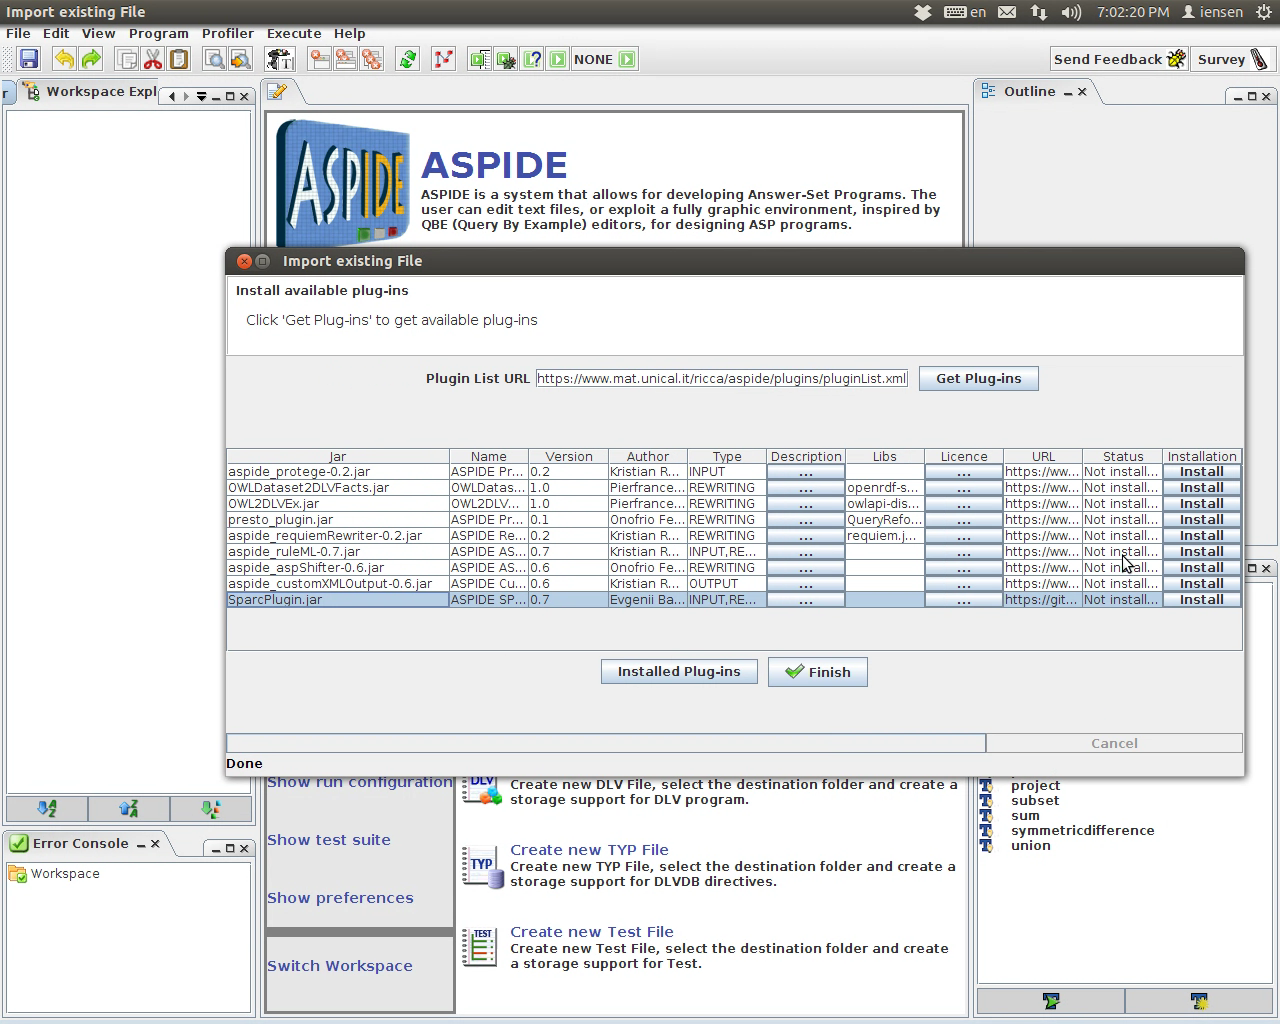
\includegraphics[width=0.9\textwidth]{plugin.png}
\caption{Installing ${\cal SPARC}$ plugin}
\label{fig:plug_install}
\end{figure}


\pagebreak
\subsection{Creating Projects and Adding  ${\cal SPARC}$  source files}
ASPIDE uses \textit{workspaces} to store projects. Workspace is a folder that can contain multiple projects. ASPIDE can have only one workspace opened, that is selected by a user when ASPIDE starts. Source files should belong to a project to be used by  ASPIDE query engine and answer set computation tools. 

\begin{itemize}
\item To create a new project, go to the menu \textit{File -\textgreater New} and select \textit{New Project} submenu. Specify the project name in the pop-up window and click on \textbf{Finish} button. You should see a new project appeared in \textbf{workspace explorer}. 
\item To add a new SPARC file, right click on the project to display context menu and select \textit{New -\textgreater File -\textgreater SPARC File} as it is shown on Figure \ref{fig:createfile} . Choose the file name in the pop-up window. You should see a new file added under the project in workspace explorer and displayed in ASPIDE editor window.
\end{itemize}

\begin{figure}[ht]
\centering
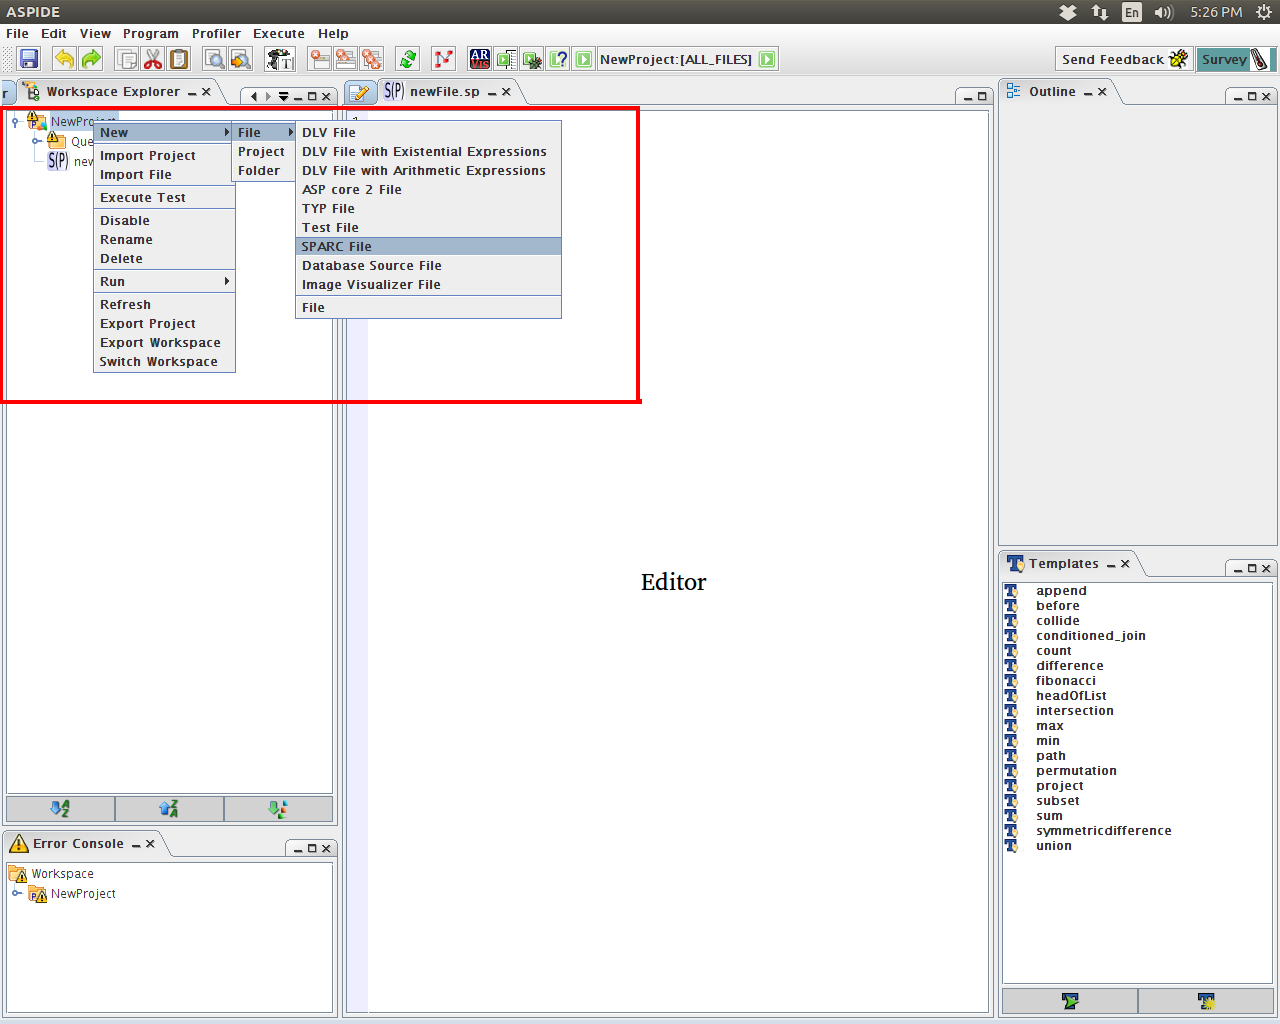
\includegraphics[width=0.9\textwidth]{project.png}
\caption{Adding  ${\cal SPARC}$ source file }
\label{fig:createfile}
\end{figure}
  
\subsection{Executing queries and computing Answer sets} 
You can execute queries and compute answer sets as for usual ASP file.
To execute a query, open a sparc file in the ASPIDE editor and click on the button with a question mark in the toolbar:
\begin{figure}[ht]
\centering
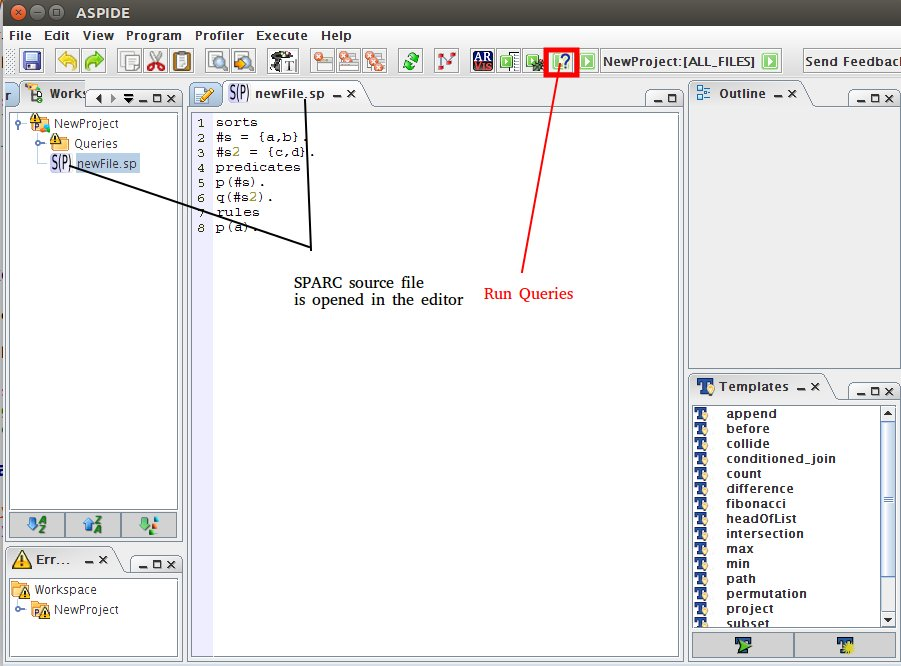
\includegraphics[width=0.9\textwidth]{openqueries.jpg}
\caption{Open Query Interface}
\label{fig:openqueries}
\end{figure}

A window will appear where you can input and run queries.
To run a query, 
\begin{itemize}
\item mark \textbf{Epistemic Mode} checkbox (this is to follow the definition of query given in the class)
\item input your query into editbox named \textbf{Query} or select one from history
\end{itemize}
The results will appear in the listview named \textbf{Results}.
See fig \ref{fig:runquery} for details.
\pagebreak
\begin{figure}[ht]
\centering
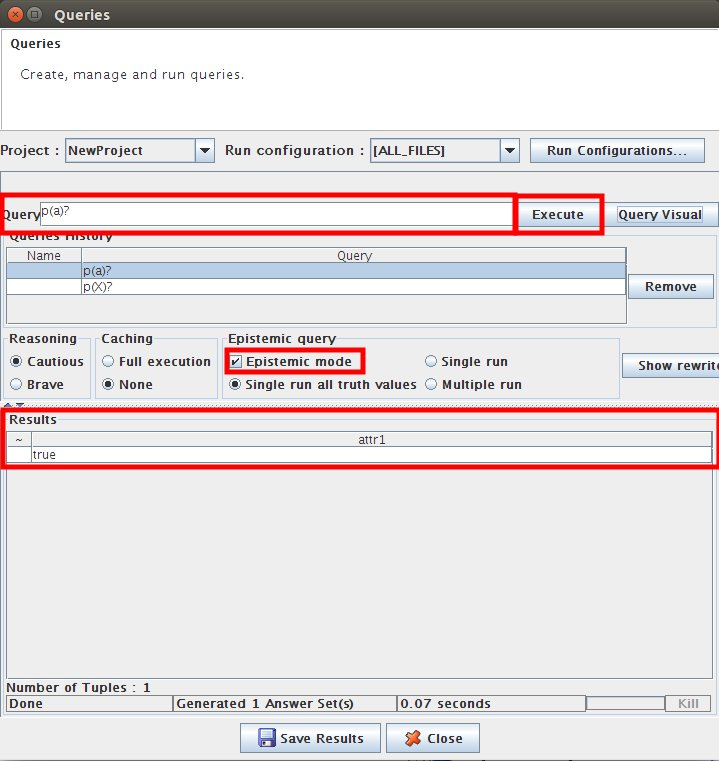
\includegraphics[width=0.9\textwidth]{runquery.jpg}
\caption{Execute a query}
\label{fig:runquery}
\end{figure}
\pagebreak

To compute answer sets of the program, press the button with green arrow marked on figure \ref{fig:ansshow}.

\begin{figure}[ht]
\centering

\includegraphics[width=0.9\textwidth]{toolbarans.jpg}
\caption{Open answer sets window}
\label{fig:ansshow}
\end{figure}

In the appeared \textbf{Run Configurations} window: 
\begin{itemize}
\item make sure a correct path to dlv in selected in \textbf{Executable} listbox. 
\item press \textbf{Run} button to see the answer sets
\end{itemize}

\begin{figure}[ht]
\centering
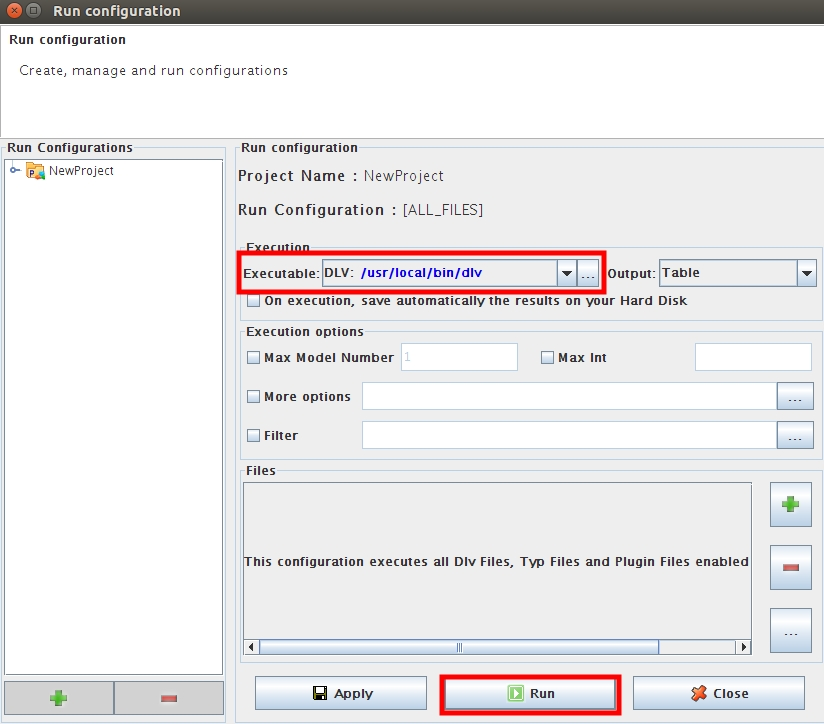
\includegraphics[width=0.9\textwidth]{answindow.jpg}
\caption{Run configurations window}
\label{fig:ansset}
\end{figure}
\pagebreak

In the displayed window, answer sets are grouped by predicate symbols in their literals.
On figure \ref{fig:ansres}, two answer sets are shown. The first one  contains two literals $p(a,b)$ and $p(e,f)$ and some literals with predicate symbol $q$.  
\begin{figure}[ht]
\centering
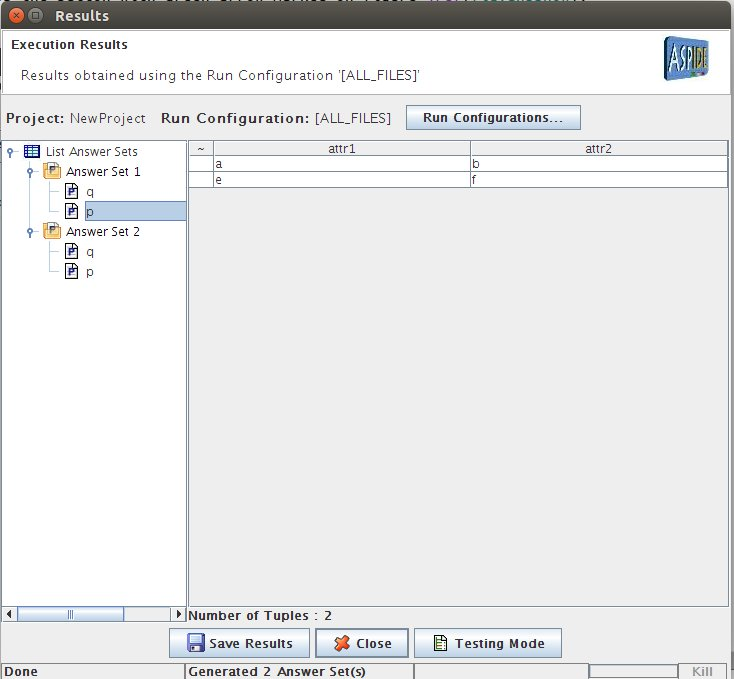
\includegraphics[width=0.9\textwidth]{results.jpg}
\caption{Answer Sets}
\label{fig:ansres}
\end{figure}



 
\subsection{Warnings Checking}

To see allow ASPIDE to show warnings (section \ref{type_warnings}), you need to install swi-prolog on your system. Swi-prolog is available from  {\scriptsize
\url{http://www.swi-prolog.org/Download.html}
} 

After swi-prolog is installed, go to the ASPIDE menu \textit{File -\textgreater Preferences}. In the appeared window select the tab \textbf{Executables/Solvers} and add a new \textit{executable} named \textit{swipl} with a path pointing to the swi-prolog executable. Usually, it is named \textit{swipl} in Unix/MacOS operating system and \textit {swipl.exe} in Windows. Click on \textbf{Save} button to close the window.
See the details on figure \ref{fig:addswipl}.
\begin{figure}[ht]
\centering
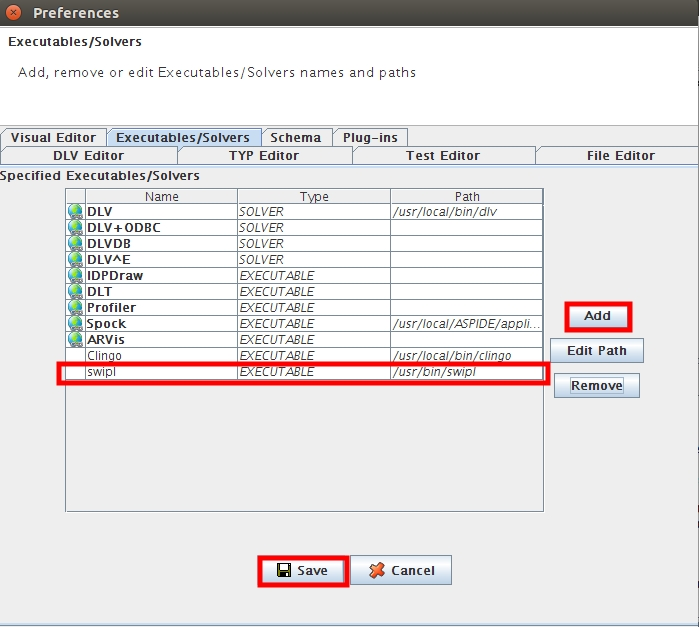
\includegraphics[width=0.9\textwidth]{swipl_add.jpg}
\caption{Adding swi-prolog executable}
\label{fig:addswipl}
\end{figure}
\pagebreak
After the executable is added, you need to specify a flag property for the ${\cal SPARC}$ plug-in to make it check warnings.
Go to ASPIDE menu \textit{File -\textgreater Plug-ins -\textgreater  Manage Plug-ins}. In the appeared window click on the cell Properties in SPARC plug-in line and add a new property \texttt{CHECK\_WARNINGS=TRUE} as it is shown on figure \ref{fig:addprop}.
Click on \textbf{Close} button to save the results.
\textbf{RESTART ASPIDE FOR THE NEW CHANGES TO TAKE EFFECT}. 

\begin{figure}[ht]
\centering
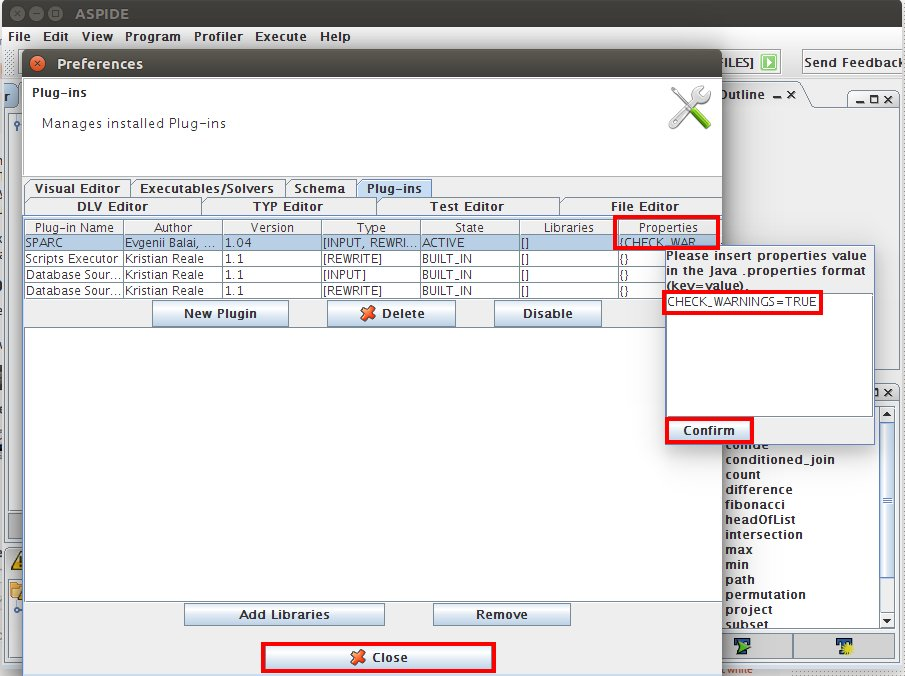
\includegraphics[width=0.9\textwidth]{property.jpg}
\caption{Adding swi-prolog executable}
\label{fig:addprop}
\end{figure}
\pagebreak
After the restart, you should be able to see the warnings in the  left lower corner of aspide interface (\textbf{Error Console}). 

\bibliography{mybib}
\bibliographystyle{plain}
\end{document}


%%% Local Variables:
%%% mode: latex
%%% TeX-master: t
%%% End:
